\chapter{The \lhcb experiment}
\chaptermark{Chapter3}
\label{chapter2}
%\addcontentsline{toc}{chapter}{The \lhcb experiment}
\lhcb is one of the four large experiments allocated at the Large Hadron Collider (\lhc). It is dedicated to the study of \CP violation and the search for new physics in rare decays of \B and \D mesons. As much focus is put on precision measurements of SM parameters as on the indirect detection of new physics that can intervene in loop and penguin diagrams.\\
The \lhc provides an ideal environment for new research in the sector of heavy flavour physics. The nominal center of mass energy of the \lhc was $\sqrt{s}=7\tev$ in 2011 and $\sqrt{s}=8\tev$ in 2012. The according \bbbar production cross sections at the hadron collider are $\sigma_{\bbbar}(7\tev)= 251.8\, \mu b$ and $\sigma_{\bbbar}(8\tev)= 291.6\, \mu b$ \cite{pythia} resulting in $6.5 \cdot 10^{11}$ \B hadrons produced in the \lhcb detector acceptance in both years combined ($3\invfb$ integrated luminosity collected in 2011 + 2012). 
Additionally to providing high statistics, the \lhc gives access to the system of the $B_s$ meson -- which was mostly beyond the reach of previous \bquark factories such as \babar and \belle \ -- allowing for the investigation of \CP violation and the search for new physics in the \Bs system.\\ 
The \lhcb collaboration has already published several new results constraining SM parameters and possible contributions from new physics, for example the restraining of SUSY parameters with the decays $B^0_s \rightarrow \mup \mun$ and $B^0 \rightarrow \mup \mun$ \cite{bsmumu}.\\
\\
This chapter is dedicated to the description of the \lhcb detector. After a general overview over the detector the different subdetectors of the tracking system and the particle identification system are presented and a summary of the detector performance is given. Then the \lhcb trigger system and different trigger lines are introduced. At the end of this chapter \lhcb software is introduced. \\
 
\section{The \lhcb detector}
\label{sec:lhcb}
The \lhcb detector was designed as a single arm forward spectrometer \cite{lhcbletter} to match the kinematics of \bbbar production shown in Figure \ref{fig:pseudorapidity}. Corresponding to this distribution, the \lhcb detector covers an angular range of $10\,$mrad$\, - \, 300 \,$mrad in the bending and $10\,$mrad$\, - \, 250 \,$mrad in the non-bending plane. Both for $7\tev$ and $8\tev$ $25\,\%$ of the produced \bbbar pairs are in the detector acceptance.\\
\\
To enable precision measurements, the \lhcb detector was build with a minimal amount of material budget. Additionally, the \lhc conducts luminosity levelling for \lhcb. The proton-beams are tuned to be displaced with respect to each other at the \lhcb collision point, giving the bunches only a small overlap while colliding. The luminosity levelling is performed in a manner that keeps the number of proton-proton interaction per bunch-crossing adjusted to an average of $1.5$ throughout the entire run.\\
\\
The \lhcb detector is composed of several subdetectors shown in Figure \ref{fig:lhcb} and presented in the following sections.
Altogether the \lhcb detector incorporates precision vertexting and tracking, worldwide leading particle identification and efficient triggering through a system of dynamic triggers.
 \begin{figure}[ht]
  \begin{center}
  \subfigure{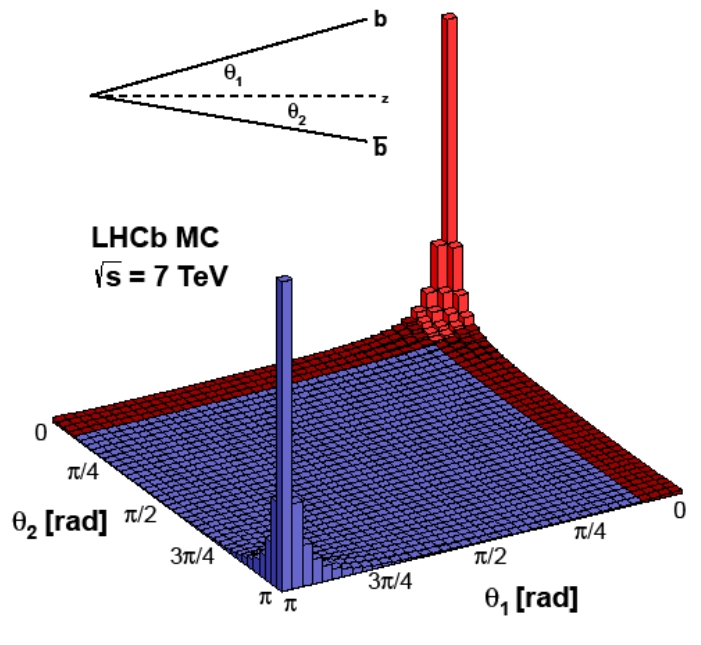
\includegraphics[width=0.4\textwidth]{pseudorapidity.jpg}}
    \subfigure{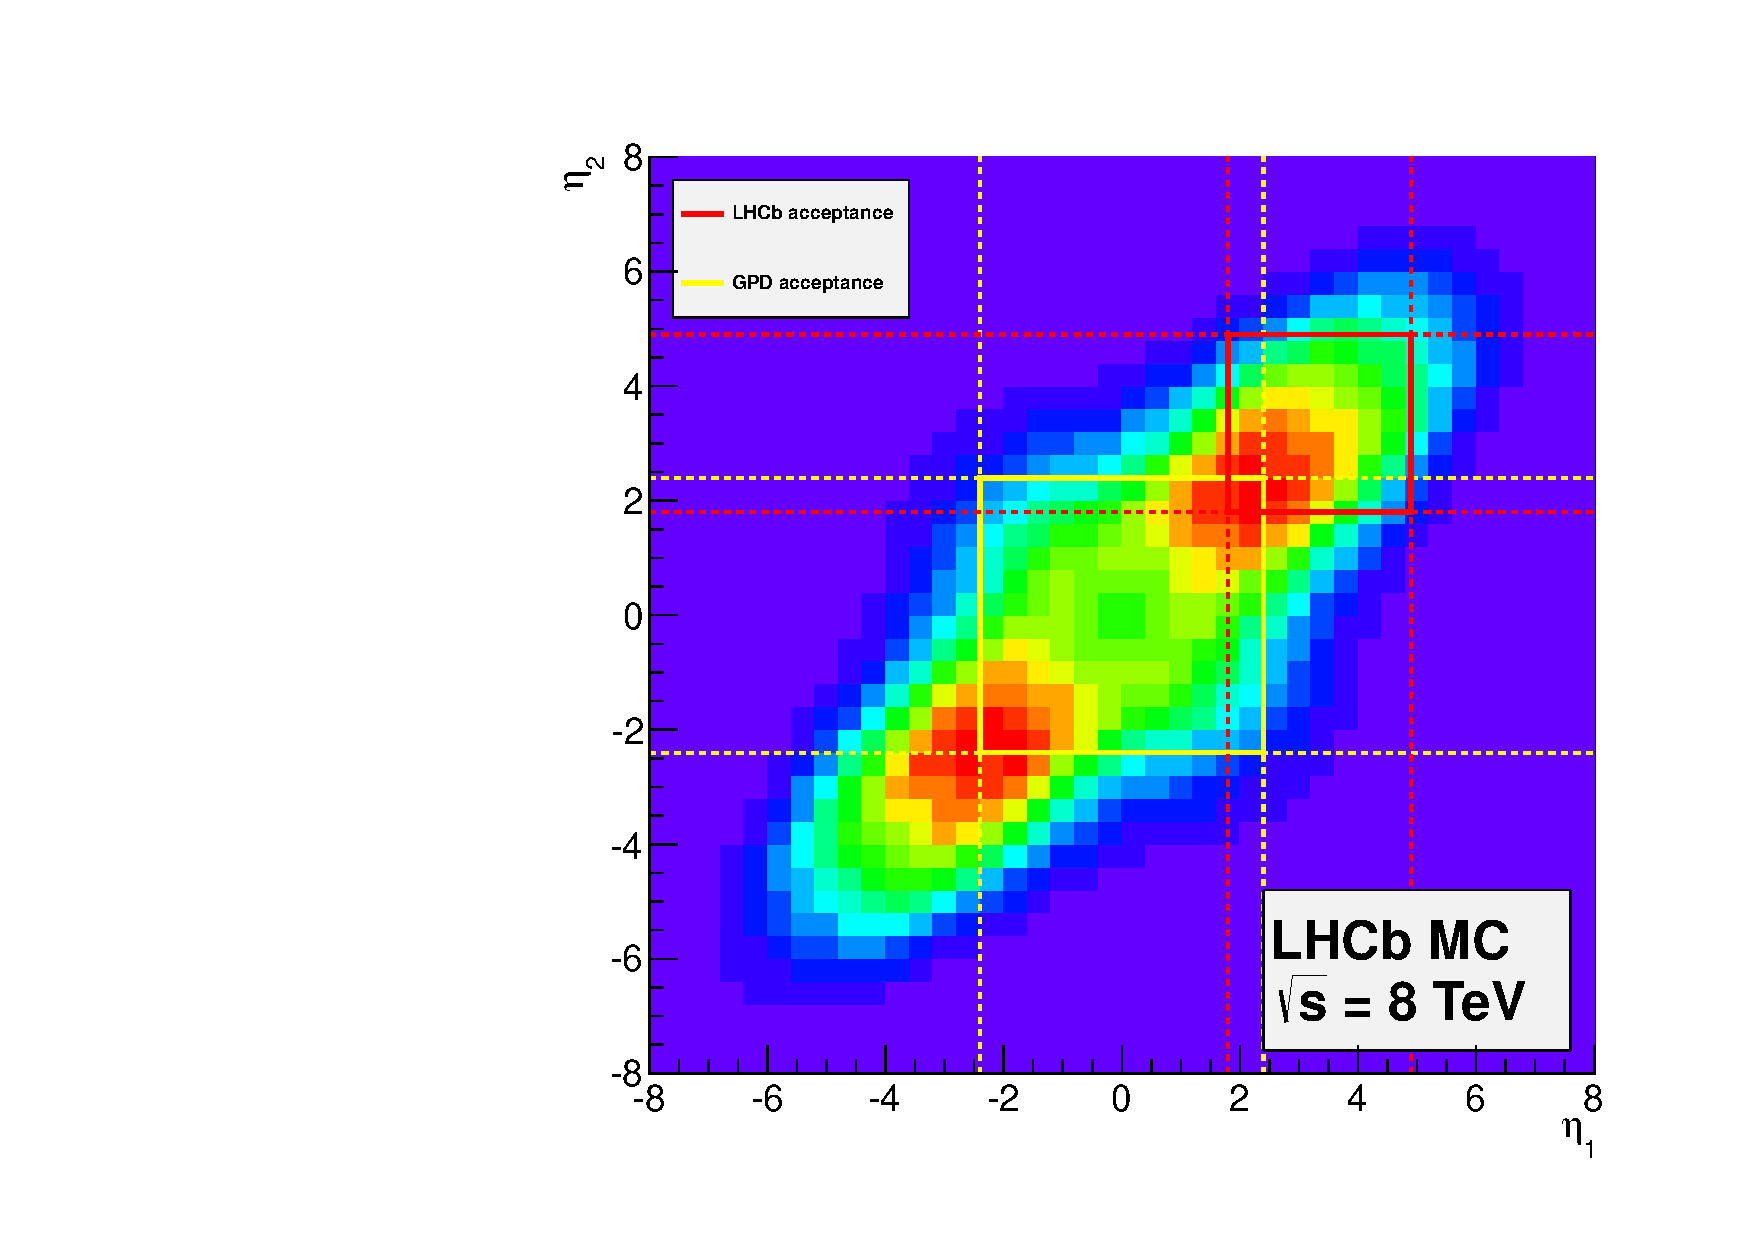
\includegraphics[width=0.42\textwidth]{acceptance.pdf}}
  \vspace*{-0.5cm}
  \end{center}
  \caption{\textit{Angular distribution of \bbbar produced in proton-proton collisions. At hadron colliders the dominant mechanism for \bbbar production is through gluon gluon fusion. Due to the statistical partition of the energy inside the protons the \bbbar pairs originated from the gluon gluon interactions are boosted in the forward or backward direction.}\cite{pythia}}
  \label{fig:pseudorapidity}
\end{figure}
\newpage

\noindent%
\begin{minipage}{\linewidth}
\makebox[\linewidth]{%
  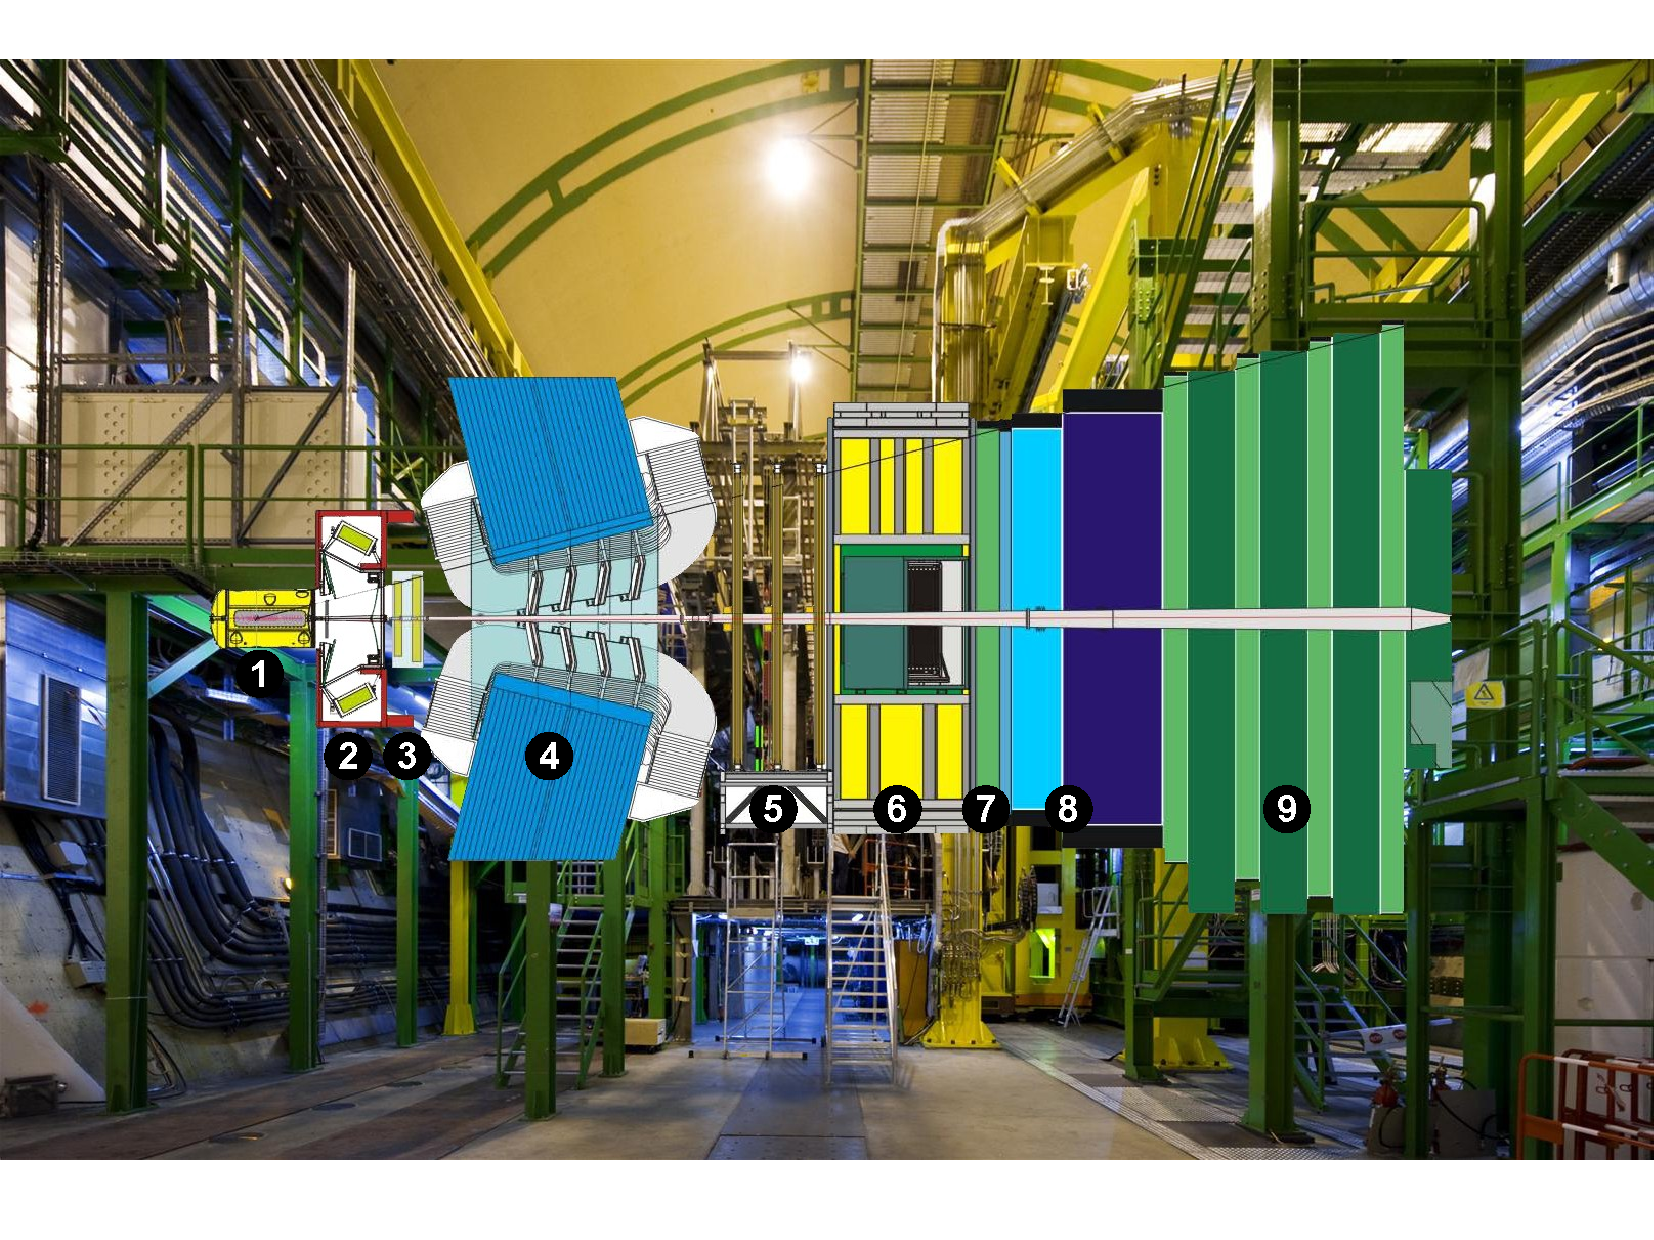
\includegraphics[angle=90, width=0.95\textwidth]{lhcb.pdf}}
\captionof{figure}{\textit{The \lhcb detector. 1: Vertex Locator (\velo), 2: Ring Imaging Cherenkov detector 1 (\richone), 3: Tracker Turicensis (\ttracker), 4: the magnet, 5: the tracking stations, 6: Ring Imaging Cherenkov detector 2 (\richtwo), 7: Muon chamber 1 (\Mone), 8: Scintillating Pad Detector (\spd), PreShower Detector (\presh), electromagnetic calorimeter (\ecal) and hadronic calorimeter (\hcal), 9: Muon chambers 2 to 5 (\Mtwo to \Mfive).}\cite{lhcb}}
  \label{fig:lhcb}
\end{minipage}
\newpage

\subsection{The tracking system}
The \lhcb tracking system's purpose is the detection of charged particle tracks and the measurement of their momenta. It is also responsible for the reconstruction of production and decay vertices of \B and \D mesons. This is essential not only for lifetime measurements but also for an efficient background rejection in the analysis of rare decays.\\
The tracking system consists of the Vertex Locator (\velo), the magnet, the Silicon Tracker (\st) and the Outer Tracker (\ot). The Silicon Tracker makes up for the entire Tracker Turicensis (\ttracker) and the Inner Tracker (\intr) which is the inner part of the three tracking stations (\Tone, \Ttwo and \Tthree) downstream of the magnet. The Outer Tracker is the outer part of the tracking stations (see 5. in Figure \ref{fig:lhcb}).
\\
%% Measure the momentum of charged particles

\subsubsection{The Vertex Locator (\velo)}
The \velo \cite{velo} accurately measures the positions of tracks close to the interaction point and allows for a very precise reconstruction of the primary vertex and the impact parameters of all tracks.\\
As shown in Figure \ref{fig:velo}, the vertex locator is approximately $1 \m$ long and consists of 21 disc-like modules arranged around the beam pipe. Each module is composed of two halfs, each having two sides with silicon strips arranged to measure the $R$ and $\Phi$ coordinate respectively. The modules can be approached as close as $8\mm$ to the beam and have a total radius of $4.2 \cm$. The strip pitch varies from $38 \mum $ wide strips nearest to the beam pipe to $102 \mum$ wide strips for the $R$ sensors and $79 \mum$ wide strips for the $\Phi$ sensors at the outer margin according to the particle density in the detector.\\
\begin{figure}[h]
  \begin{center}
  	\vspace*{-0.8cm}
    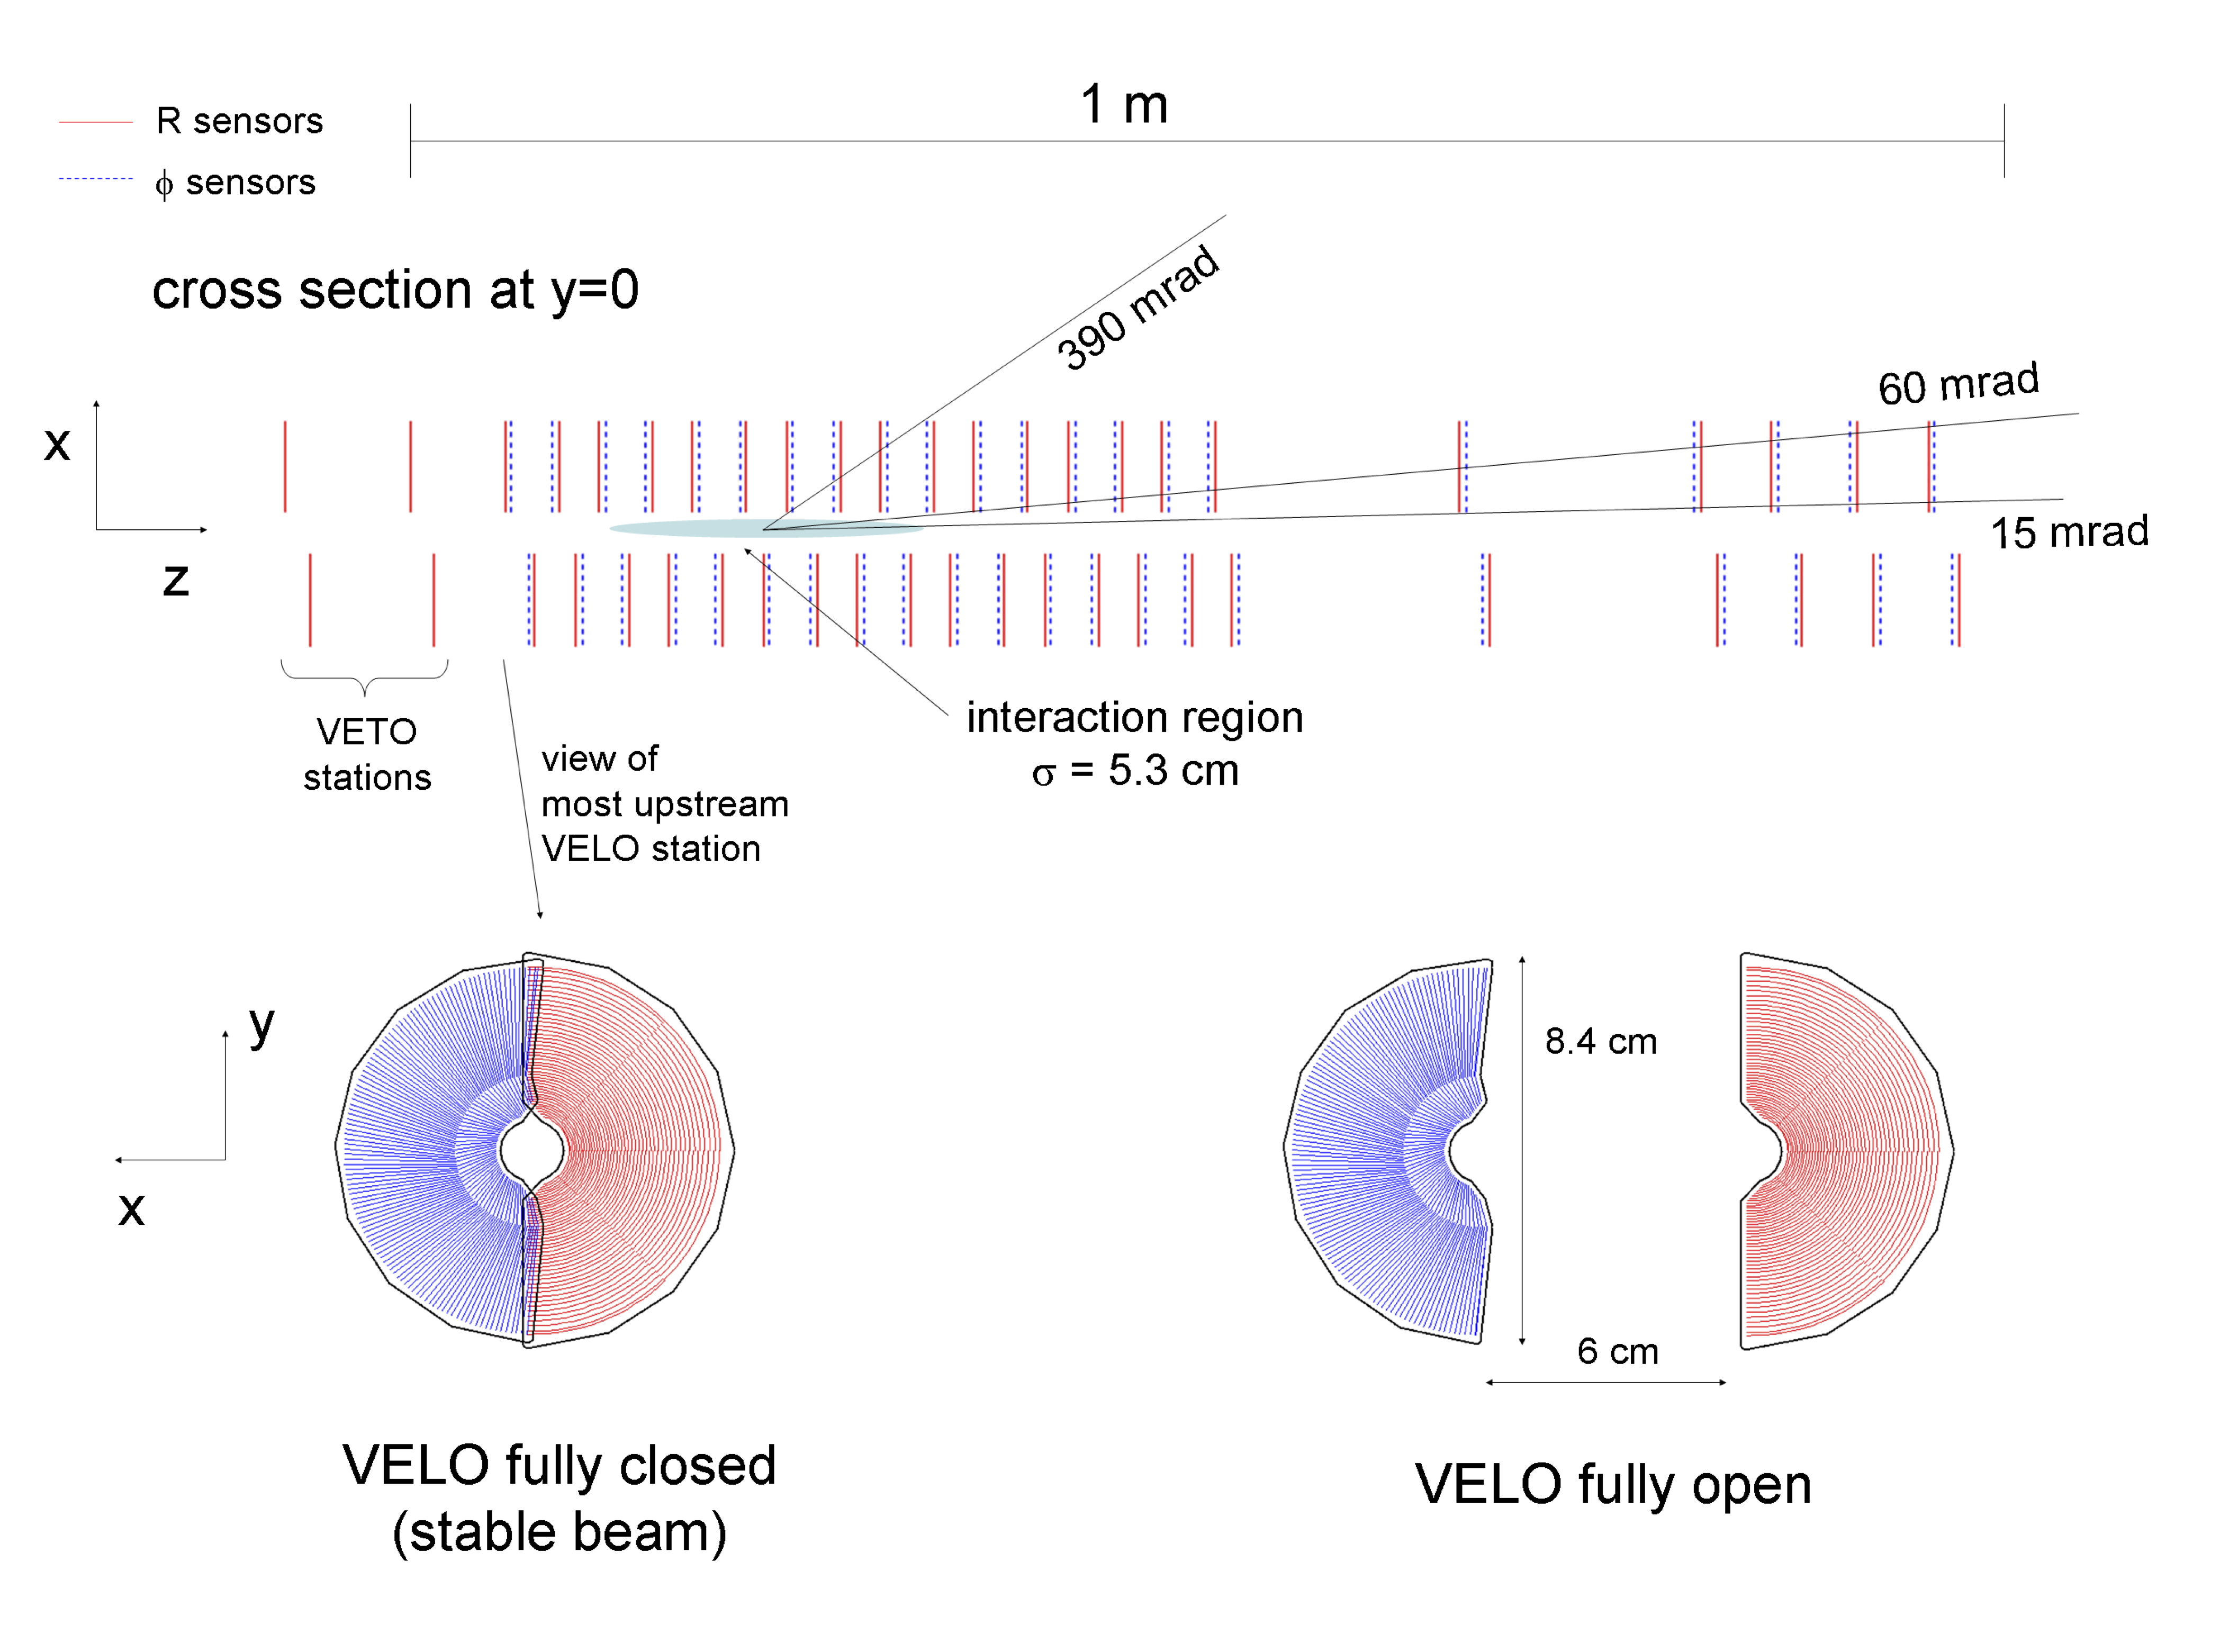
\includegraphics[width=0.75\textwidth]{velo.png}
  \vspace*{-1.0cm}
  \end{center}
  \caption{\textit{Schematic illustration of the \velo. Top: top view of the 21 modules. Bottom: Two \velo modules shown with both halfs to measure $\Phi$ (blue) and $R$ (red). Module in closed position (left) and in open position (right) which is engaged while unstable beam conditions.}\cite{velo}}
  \label{fig:velo}
\end{figure}


\subsubsection{The magnet}
The \lhcb magnet \cite{magnet} is a warm dipole magnet with saddle shaped coils. The streamlines of the magnetic field are parallel to the $y$ axis, making the $(x-z)$ plane the bending plane. Since the relative momentum resolution varies with 
\begin{equation}
\frac{\sigma_p}{p} \propto \frac{1}{B}
\end{equation}
the integrated magnetic field was chosen to be $4\, $Tm. Additionally, the magnet polarisation is regularly changed to reduce systematic effects on measurements due to geometrical acceptances.

\subsubsection{The Silicon Tracker (\st)}
The \st \cite{it} implements silicon microstrip technology for the Tracker Turicensis (\ttracker) and the Inner Tracker (\intr) with a strip pitch of about $200 \mum$. Combining the \ttracker and the \intr, the \st has four stations. Each of this four stations consists of four layers that are arranged in a $(x-u-v-x)$ geometry with vertical strips in the $x$ layers and strips rotated by a stereo angle of $-5^{\circ}$ and $+5^{\circ}$ in the $u$ and $v$ layer respectively.\\
The \ttracker is located upstream of the magnet and allows reconstruction of low momentum particles which are swept out of the detector acceptance after entering the magnetic field. It also provides information for the trigger by performing transverse momentum measurements for tracks with a large impact parameter.
With an area of $140 \cm$ width and $120 \cm$ height, the \ttracker covers the total \lhcb angular acceptance. As can be seen in Figure \ref{fig:st}, the layers of the \ttracker are divided into three different types of sectors ($K$, $M$ and $L$). According to the particle flux that is highest close to the beam pipe and drops of radially, the length of the silicon strips increases from the innermost to the outermost sensors.\\
The \intr covers the inner region of the tracking stations where the particle flux is highest. One layer of the \intr can be seen in Figure \ref{fig:st} on the right. It consists of four pieces arranged in a criss-cross pattern around the beam pipe that cover a total area of $0.35 \m^2$. 
%Each piece contains seven detector modules made out of one or two silicon sensors. The silicon sensors each carry about $400$ silicon microstrips.
\begin{figure}[ht]
  \begin{center}
  \vspace*{-0.cm}
  \subfigure{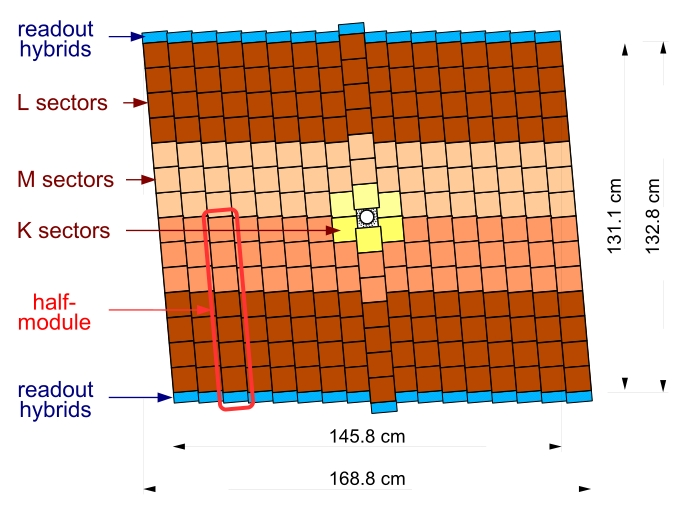
\includegraphics[width=0.49\textwidth]{tt.jpg}}
    \subfigure{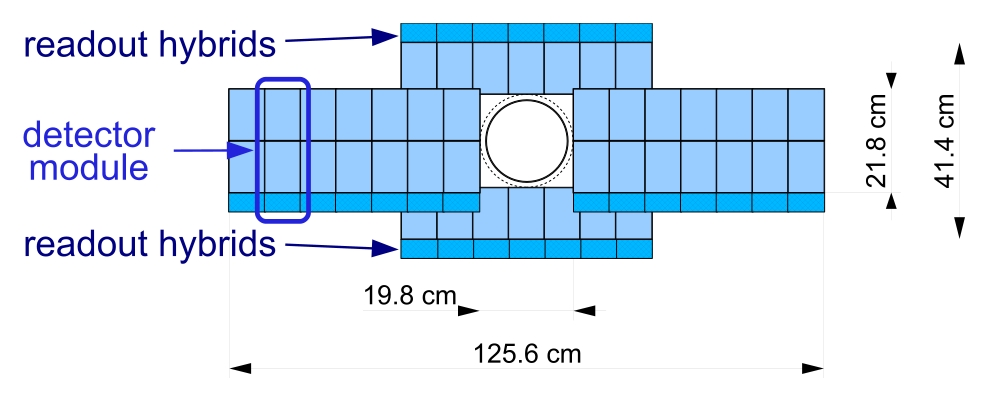
\includegraphics[width=0.49\textwidth]{it.jpg}\vspace{5cm}}
  \vspace*{-1.0cm}
  \end{center}
  \caption{\textit{The two parts of the Silicon Tracker (\st). The Tracker Turicensis (\ttracker) with the three different types of modules (left) and the Inner Tracker (\intr) which is part of the tracking stations (right).}\cite{it}}
  \label{fig:st}
\end{figure}



\subsubsection{The Outer Tracker (\ot)}
The \ot \cite{ot} covers the outer region of the tracking stations. Since the particle flux is lower in this area the \ot implements the technology of drift tubes.
As for the \st, each \ot tracking station has four layers arranged in a $(x-u-v-x)$ geometry with vertical strips in the $x$ layers and strips rotated by a stereo angle of $-5^{\circ}$ and $+5^{\circ}$ in the $u$ and $v$ layer respectively. Each layer covers the total \lhcb angular acceptance. The inner boundaries filled by the \intr were determined by the requirement that occupancies in the straw-tubes should not exceed $10\%$ at the nominal running luminosity of $2\cdot 10^{32} \cm^{-2}s^{-1}$.\\
The structure of the \ot layers is shown in Figure \ref{fig:ot}. Each layer is  build of two different types of modules. All modules are composed of two staggered layers (monolay-
\begin{figure}[ht]
  \begin{center}
  	\vspace*{-0.5cm}
    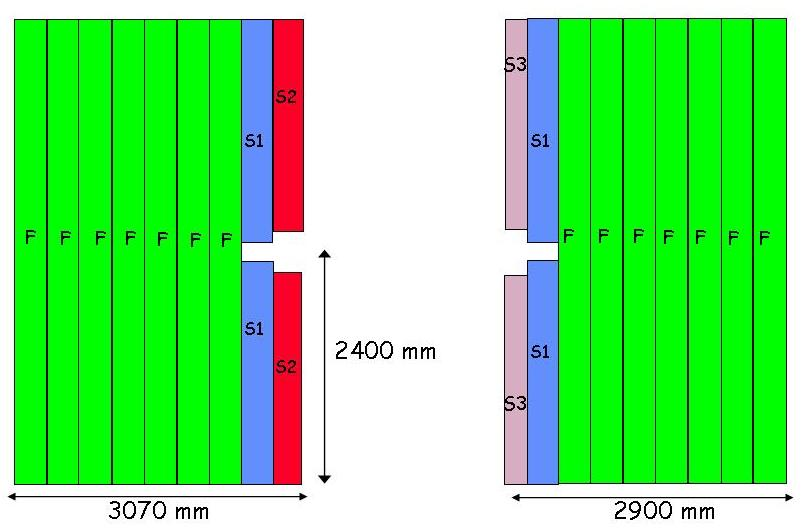
\includegraphics[width=0.45\textwidth]{OT-Modules.jpg}
  \vspace*{-0.5cm}
  \end{center}
  \caption{\textit{One layer of the Outer Tracker (\ot) with the long $F$ modules and the shorter $S$ modules combined out of $256$ and $128$ drift tubes respectively.}\cite{ot}}
  \label{fig:ot}
\end{figure}
ers) of straw-tubes.
The $F$ modules are $4.85\m$ long and consist of $256$ straw-tubes. Their monolayers are split along the $y$ axis, at different positions for each monolayer to avoid insensitive regions in the middle of the modules.
The $S$ modules are shorter than the $F$ modules and located above and below the beam pipe. Each of the $S$ modules has $128$ straw-tubes.\\
All straw-tubes are $5 \mm$ thick and filled with a gas mixture of $Argon$ and $CO_2$ ($70:30$) which combines fast response time ($<50 \ns$) with a high resolution of the drift coordinate ($200\mum$).\\


%\subsubsection{Performance}
%The \lhcb tracking system has an average relative momentum resolution of $0.5 \%$. \\
%The resolution of the $x$ and $y$ coordinates of the primary vertex and the resolution on the impact parameter's $x$ coordinate are shown in Figure \ref{fig:resolution}. For 25 tracks a resolution of $13 \mum$ on the $x$ and $y$ coordinates and a resolution of $69 \mum$ on the $z$ coordinate of the primary vertex can be reached. Additionally and equally excellent impact parameter resolution of $<35 \mum$ for tracks with a transverse momentum $p_T>1 \gev$ can be obtained.
%\begin{figure}[ht]
%  \begin{center}
%  \subfigure{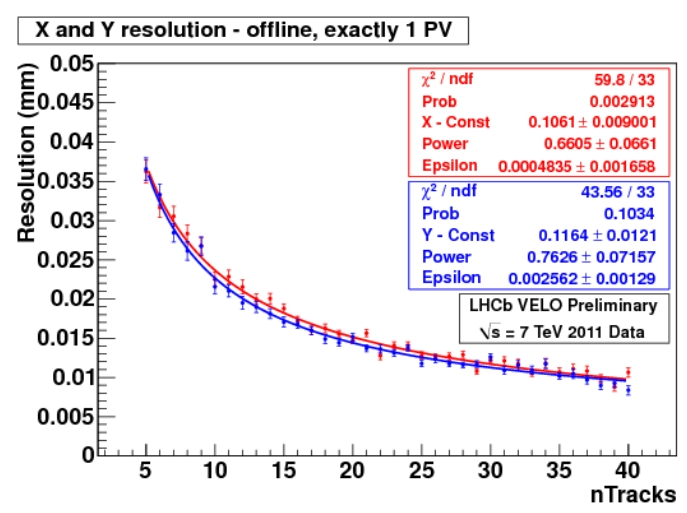
\includegraphics[width=0.45\textwidth]{PVresolution.jpg}}
%    \subfigure{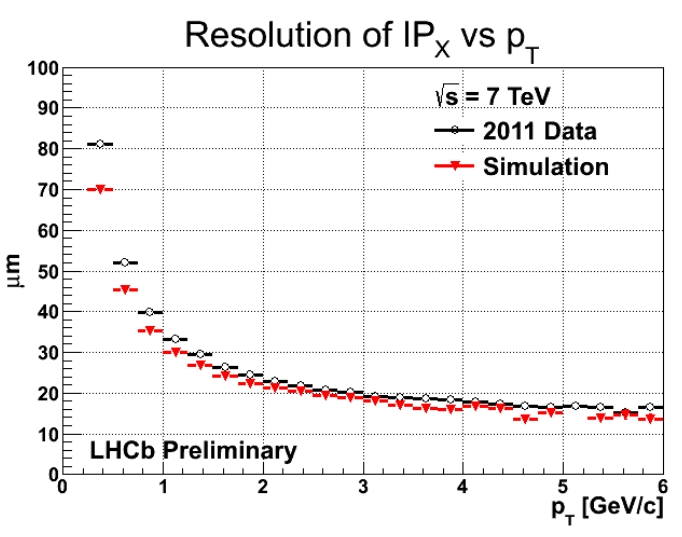
\includegraphics[width=0.45\textwidth]{IPresolution.jpg}}
%  \vspace*{-1.0cm}
%  \end{center}
%  \caption{\textit{Summary of the performance of \lhcb tracking system obtained from 2011 data and Monte Carlo. The primary vertex resolution for the $x$ and $y$ coordinates as a function of the number of tracks (left) and the of the $x$ coordinate of the impact parameter as a function of the transverse momentum $p_T$.}}
%  \label{fig:resolution}
%\end{figure}

\subsection{The particle identification system}
The \lhcb particle identification system consists of two Ring Imaging CHerenkov (\rich) detectors, the calorimeter system and the muon system. The information of these subdetectors is combined later in the offline analysis and evaluated with the use of a likelihood function.\\

\subsubsection{The \richone and \richtwo}
The \lhcb detector includes two RICHs \cite{rich} to allow for a precise separation of charged pions and kaons over the entire momentum spectrum. The separation follows through analysis of the Cherenkov light emitted by ultra-relativistic charged particles when traversing the gas of the RICHs \cite{WRLeo}.\\
\richone is placed between the \velo and the \ttracker and covers the full angular acceptance of the \lhcb detector. It uses a mixture of aerogel and $C_4F_{10}$ radiators to distinguish charged particles with a momentum between $1 \gevc \, - \, 60\gevc$.\\
\richtwo is located downstream of the magnet behind the tracking stations. It is designed to cover the momentum range from $15\gevc$ to $100\gevc$ using $CF_4$ radiator gas. Corresponding to the region where high momentum particles are produced, the \richtwo covers an angular acceptance of $15\,$mrad to $120\,$mrad (bending plane) and $100\,$mrad (non-bending plane).\\
The Cherenkov angle depending on the particles momentum is plotted in Figure \ref{fig:richrad} for different particles in the \rich radiators.
\begin{figure}[ht]
  \begin{center}
  	\vspace*{-0.5cm}
    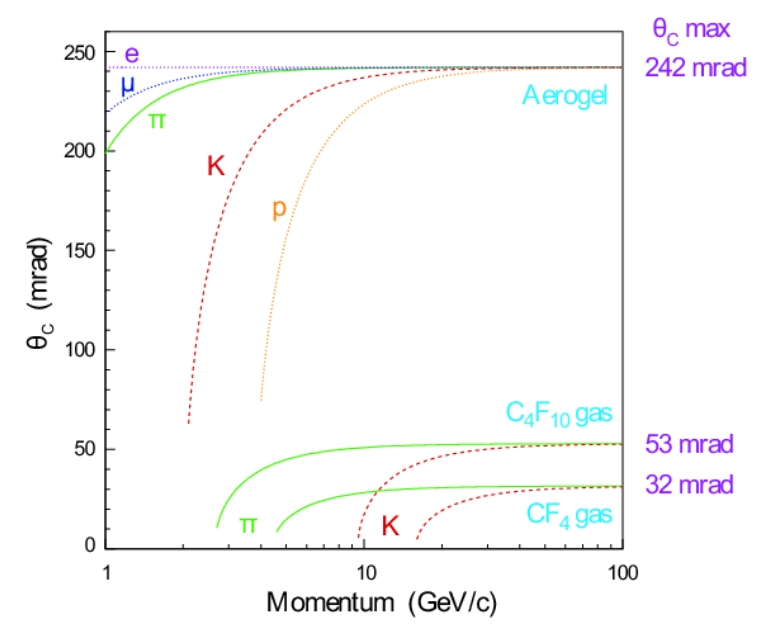
\includegraphics[width=0.55\textwidth]{richrad.jpg}
  \vspace*{-0.8cm}
  \end{center}
  \caption{\textit{Cherenkov angle versus the particle momentum for different particles in the \rich radiators.}\cite{rich}}
  \label{fig:richrad}
  \vspace*{-0.5cm}
\end{figure}

\subsubsection{The calorimeter system}
The \lhcb calorimeter system \cite{calo} consists of a Preshower detector (\presh), a Scintillating Pad Detector (\spd), an electromagnetic calorimeter (\ecal) and a hadronic calorimeter (\hcal). The main purpose of the calorimeter system is the identification of light particles such as electrons and neutral particles such as photons or \piz as illustrated in Figure \ref{fig:pid} \cite{pidcalo} and the measurement of energy and position of neutral particles that can't be detected by the tracking system. The calorimeters also provide information for the hardware based \lone trigger (see Section \ref{sec:l0}).
\begin{figure}[ht]
\vspace{-0.3cm}
  \begin{center}
    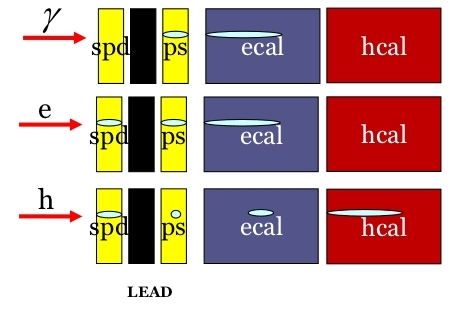
\includegraphics[width=0.5\textwidth]{CAL.jpg}
  \end{center}
  \vspace*{-1cm}
  \caption{\textit{Schematic illustration of the particle separation using the calorimeter system. The lead layer between the Scintillation Pad Detector (\spd) and the PreShower detector (\presh) is thick enough to induce electromagnetic showers.}\cite{calo}}
  \label{fig:pid}
  \vspace*{-0.5cm}
\end{figure}
% but too thin to start a significant hadronic shower

Each subdetector of the calorimeter system is composed of square cells varying in size according to the particle flux. For the \spd, \presh and the \ecal three different zones were chosen with cell sizes of $4\cm$, $6\cm$ and $12\cm$ as shown in Figure \ref{fig:calo}. The \hcal is segmented into two zones with larger cells ($13.13\cm$ in the inner section and $26.26\cm$ in the outer section) because of the size of hadronic showers. All calorimeters implement the technology of scintillation light that is transmitted to Photo-Multipliers (PMT) by wavelength-shifting (WLS) fibres.\\
\begin{figure}[ht]
  \begin{center}
  	\vspace*{-0.8cm}
    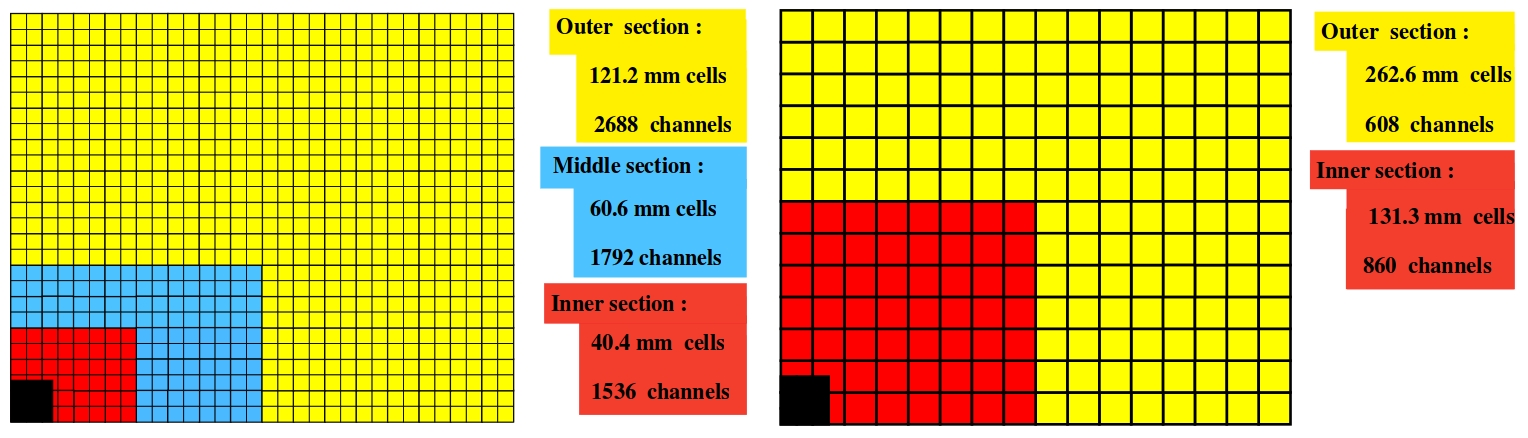
\includegraphics[width=0.85\textwidth]{calocells.jpg}
  \vspace*{-0.5cm}
  \end{center}
  \caption{\textit{Schematic illustration of the segmentation of the Scintillating Pad Detector (\spd), PreShower detector (\presh) and the \ecal (left) and the \hcal (right). The pictures show one quarter of the calorimeter surfaces. The black area on the bottom left of both images is the area close to the beam pipe where the particle flux is too high for any calorimeter performance.}\cite{calo}}
  \label{fig:calo}
  \vspace*{-0.5cm}
\end{figure}

The \presh and the \spd are located before the \ecal and separated by lead sheet of $2.5 \, \Xrad$ thickness allowing for a separation of electrons from a high background of pions. Both \presh and \spd are made of one single layer of $15\mm$ thick plastic-scintillator tiles.\\
The \ecal is composed of cells that are build after the shashlik  principle, one cell is composed of alternating layers of $2\mm$ thick lead and $4\mm$ thick polystyrene scintillator tiles. One cell, made out of 66 lead and scintillator layers, is illustrated in Figure \ref{fig:calos}.
The \hcal employs a non-typical structure where the scintillating tiles are arranged parallel to the beam pipe as shown in Figure \ref{fig:calos}. The absorber for the \hcal was chosen to be $1\cm$ iron tiles and the scintillator layers are made out of $3\mm$ thick doped polystyrene tiles.
\begin{figure}[ht]
  \vspace*{-0.5cm}
  \begin{center}
  \subfigure{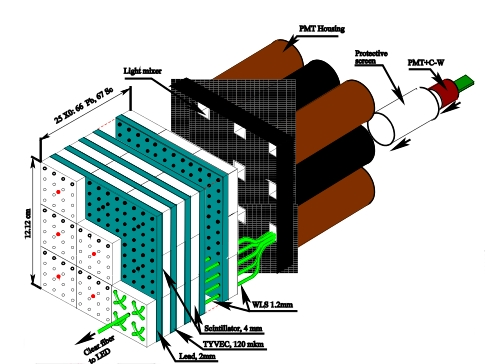
\includegraphics[width=0.45\textwidth]{ECAL.jpg}}
   \subfigure{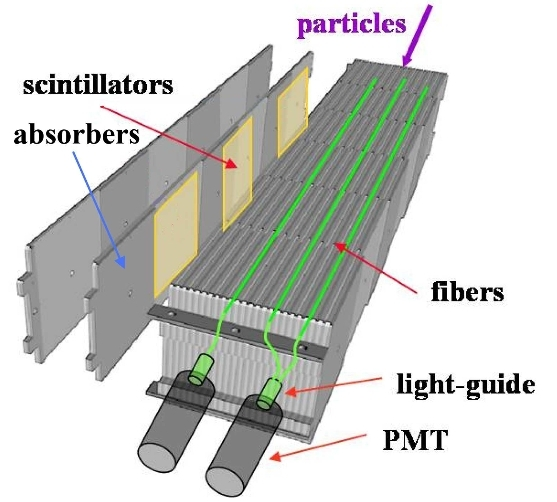
\includegraphics[width=0.43\textwidth]{hcal1.jpg}}
  \vspace*{-0.8cm}
  \end{center}
  \caption{\textit{One cell of the \ecal (left) and the \hcal (right). The scintillating tiles of the \ecal are arranged perpendicular to the beam while they are parallel to the beam for the \hcal. The absorber is made of lead for the \ecal and iron for the \hcal.}\cite{calo}}
  \label{fig:calos}
\end{figure}


\subsubsection{The muon chambers}
The \lhcb detector contains five muon stations (\Mone - \Mfive) dedicated to muon identification and muon triggering \cite{muon}.\\
The first muon station \Mone is placed upstream of the calorimeters to provide a precise transverse momentum measurement. The other muon stations are placed downstream of the calorimeters and interleaved with $80\cm$ thick iron absorbers. The stations \Mtwo and \Mthree yield a very good spacial resolution for the tracks while the last two stations only deliver information for the particle identification. The side view of the muon system is shown in Figure \ref{fig:muons}.\\
As can be seen on the left in Figure \ref{fig:muons}, each muon chamber is divided into four regions R1 to R4. The granularity in the regions decreases radially which provides an isotropic channel occupancy for each muon station. Except for the inner region R1 of \Mone, all muon stations are composed of Multi Wire Proportional Chambers (MWPC). R1 of \Mone implements the Triple GEM \cite{gem} technology because the particle flux in this region would overburden the MWPC.\\
\begin{figure}[ht]
\vspace*{-0.5cm}
  \begin{center}
  \subfigure{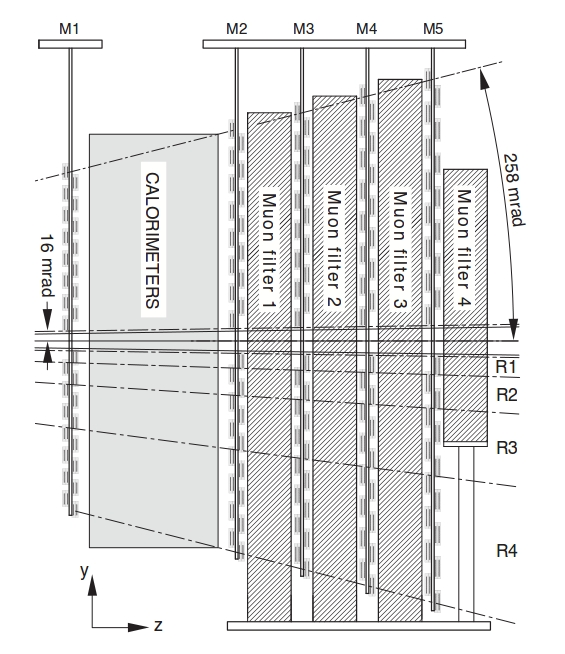
\includegraphics[width=0.35\textwidth]{muon2.jpg}}
   \subfigure{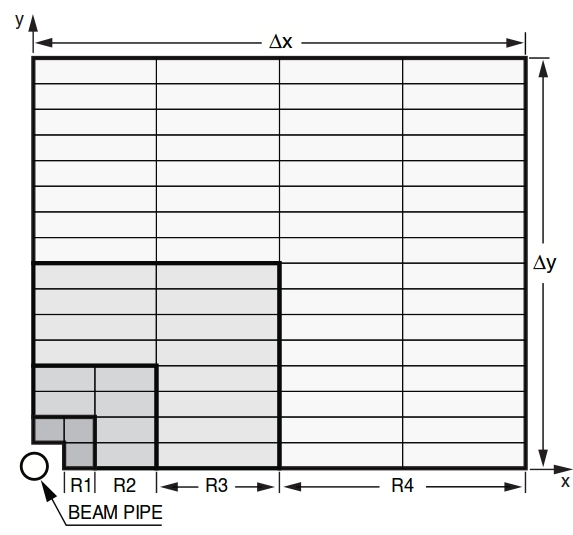
\includegraphics[width=0.35\textwidth]{muon1.jpg}}
  \vspace*{-1.0cm}
  \end{center}
  \caption{\textit{Side view of the muon stations (left) and the schematic front view of the upper right quarter of one muon station with the segmentation into four regions R1 to R4. All modules are composed of MWPC except for R1 of M1 which uses the Triple GEM technology due to extremely high particle flux.}\cite{muon}}
  \label{fig:muons}
\end{figure}

\subsubsection{The discriminant particle identification variable}
\label{sec:pid}
The information from the detectors of the particle identification system is used in the offline analysis to calculate a discriminative variable $\mathrm{DLL}$. This variable is calculated for all final state tracks. It is computed by testing the hypothesis that a track is a certain particle with respect to the hypothesis that the track comes from another particle. The reference particle is usually chosen to be a pion.\\
The information on the particle identification variable for kaons and pions (\dllkpi) comes mainly from the \richone and \richtwo. For neutral particles and electrons (\dllepi) the calorimeter system provides the significant information while the particle identification variable for muons (\dllmupi) is calculated by relying especially on the muons system.\\

\subsection{\lhcb performance summary}
The \lhcb detector has shown a high and stable performance over the entire range of data taking \cite{lhcbperf}.\\
%The primary vertex resolution obtained by the \velo is $13 \mum$ for the $x$ and $y$ coordinates and $69 \mum$ for the $z$ coordinate for an average of $25$ tracks coming from the primary vertex \cite{veloperf} \cite{tsperf}. An equally excellent impact parameter resolution of $<35 \mum$ for tracks with a transverse momentum $p_T>1 \gev$ can be obtained. The resolution of the $x$ and $y$ coordinates of the primary vertex and the resolution on the impact parameter's $x$ coordinate are shown in Figure \ref{fig:resolution}. 
%The \lhcb tracking system has an average relative momentum resolution of $0.5 \%$. \\
The resolution of the $x$ and $y$ coordinates of the primary vertex and the resolution on the impact parameter's $x$ coordinate are shown in Figure \ref{fig:resolution}. For 25 tracks a resolution of $13 \mum$ on the $x$ and $y$ coordinates and a resolution of $69 \mum$ on the $z$ coordinate of the primary vertex can be reached \cite{veloperf}. Additionally an equally excellent impact parameter resolution of $<35 \mum$ for tracks with a transverse momentum $p_T>1 \gev$ can be obtained. The tracking system has an average relative momentum resolution of
\begin{equation}
\frac{\Delta p}{p} = 0.5 \% \quad \cite{tsperf}.
\end{equation}
The relative energy resolution for the \ecal is
\begin{equation}
\frac{\Delta E}{E} = \frac{10 \%}{\sqrt{E[\gevc]}} \oplus 1\%
\end{equation}
and for the \hcal
\begin{equation}
\frac{\Delta E}{E} = \frac{80 \%}{\sqrt{E[\gevc]}} \oplus 10\%
\end{equation}
\\
The particle identification system has varying performances for different particle types and momenta. For example, the average electron identification efficiency is $90\%$ for a $5\%$ misidentification rate. The average kaon identification efficiency is $95\%$ for a $5\%$ rate of misidentifying a pion as a kaon.
\begin{figure}[ht]
  \begin{center}
  \subfigure{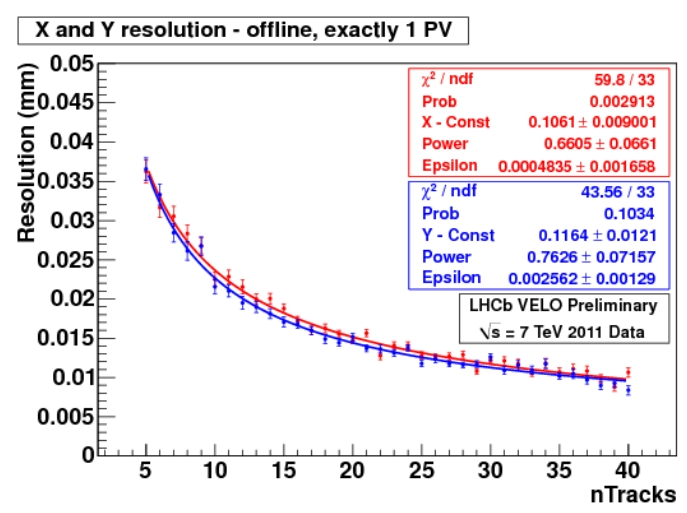
\includegraphics[width=0.49\textwidth]{PVresolution.jpg}}
    \subfigure{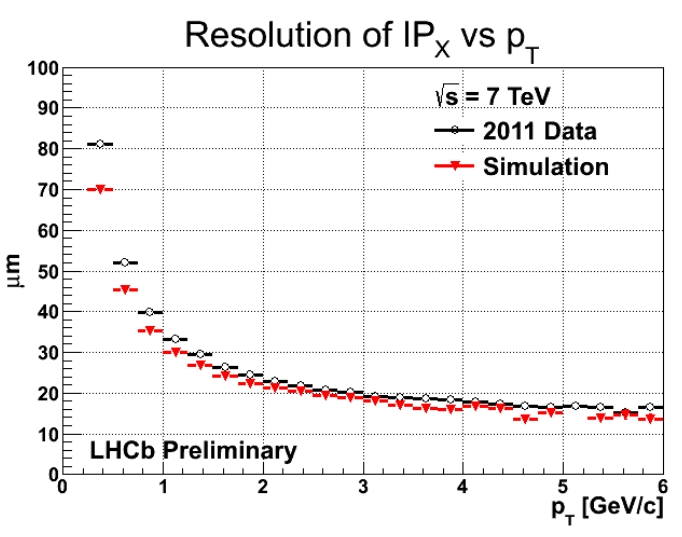
\includegraphics[width=0.49\textwidth]{IPresolution.jpg}}
  \vspace*{-1.0cm}
  \end{center}
  \caption{\textit{Summary of the performance of \lhcb tracking system obtained from 2011 data and Monte Carlo. The primary vertex resolution for the $x$ and $y$ coordinates as a function of the number of tracks (left) and the of the $x$ coordinate of the impact parameter as a function of the transverse momentum $p_T$.}\cite{veloperf}}
  \label{fig:resolution}
\end{figure}
\newpage
%
%
%
\vspace{0.5cm}
\section{The trigger system}
The \lhc collides bunches at a rate of $40 \mhz$. Due to the \lhcb's luminosity levelling the visible\footnote{To be visible, events must have at least two charged particles producing enough hits in the tracking system to be reconstructed.} rate of interaction is $10\mhz$ which has to be reduced to about $4\khz$ to be permanently stored for offline analysis. At \lhcb this is realized by a two-stage trigger system \cite{trigger} \cite{trigger2}: the Level-0 (\lone), a purely hardware based trigger, followed by the High Level Trigger (\hlt) which is executed on a processor farm. A schematic presentation of the trigger system can be seen in in Figure \ref{fig:trigger}.
\begin{figure}[ht]
\vspace*{-0.3cm}
  \begin{center}
    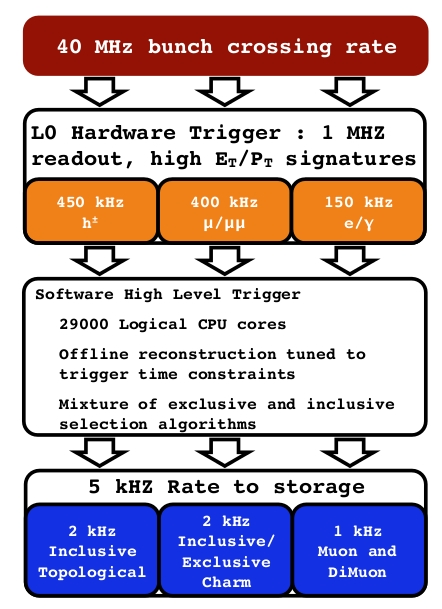
\includegraphics[width=0.43\textwidth]{trigger.jpg}
  \vspace*{-0.5cm}
  \end{center}
  \caption{\textit{A schematic representation of the \lhcb trigger system. The first state is the hardware based Level-0 trigger. Afterwards the High Level Triggers are executed on a processor farm. Each subtrigger uses several trigger lines for dynamic and specific triggering.}}
  \label{fig:trigger}
\end{figure}


\subsection{The Level-0 trigger}
\label{sec:l0}
The \lhcb Level-0 (\lone) trigger is made from custom electronics and reduces the rate from $10\mhz$ to $1\mhz$.\\
To identify events from \B hadrons the \lone trigger makes use of the fact that the large mass of \B hadrons provides a significant amount of transverse kinetic energy to the decay particles. Therefore it selects events with a high amount of transverse energy deposited in the calorimeter or the muon system. Additionally, the \lone accesses information from the \velo pileup and the \spd to reject events with too many tracks. There are different \lone trigger lines for different particles. The two lines important for the analysis are the \lone Electron and the \lone Hadron which will be presented in the following.\\
% Within the bandwidth allocated to the electron trigger (cf. section 7.1.2) the electron Level 0 trigger is required to reject 99\% of the inelastic pp interactions while providing an enrichment factor of at least 15 in b events. This is accomplished through the selection of electrons of large transverse energy ET.  and the \lone TIS (Trigger Independent of Signal)
\newpage
\textbf{The \lone Electron} trigger line is fired by one electromagnetic cluster ($2\times 2$ \ecal cells) with a transverse energy $E_T$ above a threshold value. The electromagnetic cluster must have at least one corresponding hit in the \spd to identify a charged particle opposed to a photon. The threshold value for the transverse energy of the electromagnetic cluster has changed several times over the years 2011 and 2012. This will be evaluated further in Chapter \ref{Chapter4} in Section \ref{sec:triggercat}.\\
\textbf{The \lone Hadron} trigger line is activated by one cluster in the \hcal. The threshold transverse energy $E_T$ for the \lone Hadron is the sum of the transverse energy in the \hcal with the transverse energy the corresponding \ecal cells.
\\
\subsection{The High Level Trigger}
\label{sec:hlt}
All events that pass the \lone trigger will be passed on to the High Level Trigger (\hlt). The \hlt is divided into two levels (\hltone and \hlttwo) which are both implemented as a set of \cpp algorithms run on a CPU farm.\\
\\
Additionally to the information available to the \lone, the \hltone has access to information from the \velo and the tracking system. It reconstructs particles in the \velo and determines the position of the primary vertices in each event. The \hltone then makes a decision based upon impact parameter, momentum, transverse momentum and/or track quality of one track in the event.\\
For each \lone line several \hltone lines are executed. The \hltone reduces the rate to approximately $40 \khz$.\\
\\
All events that pass the \hltone go through to the \hlttwo that performs an event reconstruction similar to the offline analysis. Starting by reconstructing all tracks in the event using the \velo tracks as seed, the \hlttwo reconstructs intermediate particles and resonances and identifies displaced vertices. Afterwards, depending on the \hlttwo line, different sets of selections are applied which are dominantly designed to identify decays of \B and \D hadrons. The \hlttwo finally reduces the rate to about $4\khz$ which is stored for the offline analysis.\\
\\
One \hltone line and several \hlttwo lines will be used in the analysis of the\\ \BdKstee decay. The \hltone line that is used, is the  \textit{Hlt1TrackAllL0Decision} line. This line selects events with at least one track with a high transverse momentum $p_T$ and a great impact parameter (IP) with respect to the primary vertex, since this track is likely to come from a decaying \B hadron.\\
The \hlttwo lines that are used are the \textit{\hlttwo topological lines} \cite{hlt2topo}. These have been designed to trigger inclusive $n$-body ($n = 2,3,4$) \B decays. The \hlttwo lines implement a $Boosted Decision Tree$ to determine if $n$ tracks show the topology of a \B decay. Missed tracks are compensated for by tacking into account the difference between the total momentum of the $n$ tracks and the momentum of the hypothetical \B hadron.\\
\newpage

\section{The \lhcb stripping}
In order to reduce computing time, all events are preselected by a certain \textit{stripping line}. A stripping line consists of a loose selection aiming at rejecting as much background as possible while keeping as much signal as possible. Each decay studied at \lhcb has its own stripping line. All stripping lines are run on the entire dataset regardless of the trigger decision. The stripping is executed by the physics analysis software \davinci (see Section \ref{sec:software}).\\
During the stripping procedure every event is scanned for tracks that can be combined (see Chapter \ref{chapter3}) to make the signal decay. Events with signal candidates are stored for later use.\\

\section{The \lhcb software}
\label{sec:software}
The data processing at \lhcb goes through a series of steps which are executed by different software frameworks. To ensure consistency between these frameworks and the way that data and Monte Carlo are treated, all \lhcb core software is embedded in the \gaudi framework \cite{gaudi}.\\
There are four main applications, each responsible for a different stage of event processing:
\\
\begin{itemize}
\item \textbf{\gauss}is used for the generation of Monte Carlo. Therein, proton-proton collisions are simulated with \pythia \cite{pythia}, the decay of \B hadrons is made with \evtgen \cite{evtgen} and the detector simulation is implemented in \geant \cite{geant}.\\
\item \textbf{\boole}takes the output from \gauss and simulates the digitization of data to give it the same format as the \lhcb data obtained by the electronics and data acquisition systems.\\
\item \textbf{\brunel}performs subdetector and global reconstruction using pattern recognition for both Monte Carlo and real data.\\
\item \textbf{\davinci}executes the last step, namely the reconstruction of the final signal events and running the stripping \cite{davinci}(more details in Chapter \ref{chapter3}).
\end{itemize}

%\textbf{The \lone TIS trigger line}
%All decays that were not triggered by one of their own tracks but later on selected by the Stripping (see Section \ref{sec:stripping}) are called TIS events because the events was triggered independently from the signal by another track in the events, coming from the other \B hadron for example. The \lone TIS decays are most free from any trigger systematics and the trigger efficiency is independent of the decay which is absolutely not the case for the other trigger lines.\\